
\part{Setting up a Game}
\label{setting_up_a_game}

\section{Building an Army}
\label{building_an_army}

\nameofthegame{} includes a series of Army Books which contain descriptions of the different armies. Each army has unique Characters, troops, and rules. All unit entries within an Army Book are divided between different Categories, which may be constrained to represent a minimum or maximum percentage of the \hyperref[army_points]{Army Points}.

The first step to build an army is to write down a selection of units, options, and their Point Costs on a document, called the Army List. The exact composition of an army is subject to certain rules and restrictions which this chapter will describe in detail.

\subsection{Point Costs}
\label{point_costs}

Each unit, weapon, upgrade, Special Equipment, etc. costs a certain amount of points. A unit's Point Cost is the sum of its starting Point Cost and the Point Costs of all its additional models and upgrades. An army's Point Cost is the sum of all its units' Point Costs.

\section{Army List Structure}
\label{army_list_structure}

Each army is subdivided into several Categories. These Categories ensure that armies used in the game can represent vastly different modes of play. This could represent a single Character and its hunting party or large armies numbering in their thousands clashing for the fate of the world. They still restrict the selection in such a way to enable players to enjoy a balanced gaming experience.

An army in \nameofthegame{} is subject to basic composition rules detailed in this section.

\subsection{Army Points}
\label{army_points}

Before building an army, decide with your opponent on the size of the battle, quantified by the Army Points. The combined points value of every unit in your army, including options and equipment, must not exceed the Army Points. An army may fall below the limit only by 40 points or less.

\subsection{Army Categories}
\label{army_categories}

The Army List from which the structure of each fighting force is derived is divided into Army Categories. Every unit on the Army List belongs to one or more Army Categories. The number of points one can spend on each of these Army Categories is defined in each Army Book individually. The Army Category to which a unit belongs is marked with one or more icons in the unit entry in the Army Book.

The Army Categories are divided into three broad and sometimes overlapping groupings: the commanders and the outstanding (Characters), the backbone (Core and Special), and the thematic additions or classifications (Army Specific). All armies must have units from the Characters and Core Army Categories in their army roster.

\newpage
\subsubsection{Characters}

\begin{itemize}[label={-}]
\item This Army Category always has a maximum amount of points that can be spent on it, usually around \SI{40}{\percent} of the Army Points.
\item Unless noted otherwise, entries that belong to this Category follow the rules for Characters given in \totalref{characters}.
\end{itemize}

\begin{minipage}[c]{0.17\textwidth}
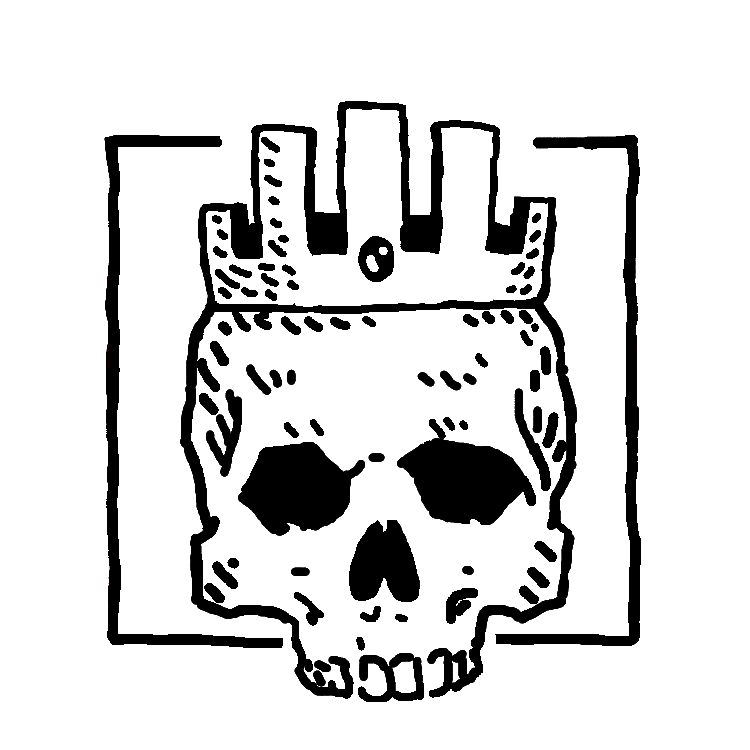
\includegraphics[width=\textwidth]{../Layout/pics/logo_character.png}
\end{minipage}\hfill
\begin{minipage}[c]{0.80\textwidth}
\flufffont{Characters represent the leaders and exceptional individuals who, through their particular sets of skills, influence the course of battle using either brute force, tactical acumen, spell casting ability, or engineering knowledge. It is they who muster the army, and your force will always include at least one representative of this Category to serve as your army General.}
\end{minipage}

\subsubsection{Core}

\begin{itemize}[label={-}]
\item This Army Category always has a minimum amount of points that must be spent on it, usually around \SI{25}{\percent} of the Army Points.
\end{itemize}

\begin{minipage}[c]{0.17\textwidth}
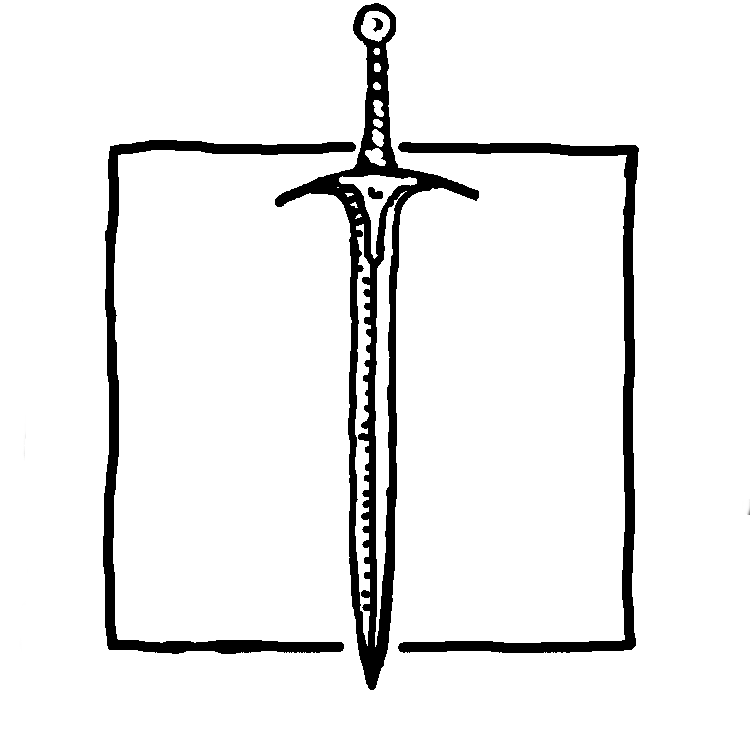
\includegraphics[width=\textwidth]{../Layout/pics/logo_core.png}
\end{minipage}\hfill
\begin{minipage}[c]{0.80\textwidth}
\flufffont{The Core represents the most readily available warriors a faction has access to and will form the bulk of combatants under the command of the Characters in the force. No matter where or why the faction fights, the Core are those units that will always be present in some combination as part of the fighting force. They are also those warriors that a society can provide for battle in the greatest numbers. While armies can overwhelmingly be formed out of the Core units, it is rarely the case as each commander seeks to deploy a force that contains as many of their finest or more specialised warriors as possible, depending on the resources available to them.}
\end{minipage}

\subsubsection{Special}

\begin{itemize}[label={-}]
\item This Army Category has neither a maximum nor a minimum limit. You are free to spend any amount of points on units in this Category, provided the obligatory sections of the army roster are filled.
\end{itemize}

\begin{minipage}[c]{0.17\textwidth}
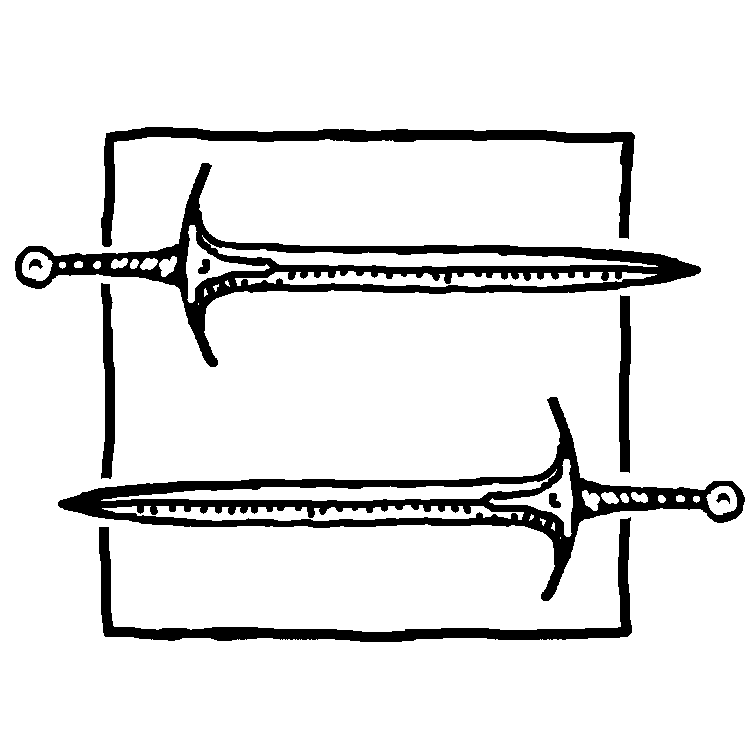
\includegraphics[width=\textwidth]{../Layout/pics/logo_special.png}
\end{minipage}\hfill
\begin{minipage}[c]{0.80\textwidth}
\flufffont{The Special Category represents more specialised warriors. A faction can call upon large numbers of these warriors and they can often be the most numerous segment of the entire fighting force. However, their numbers are still limited, and though some of these units can form an entire battle line there just isn't enough of them to form armies on their own.}
\end{minipage}

\subsubsection{Army Specific}

\begin{itemize}[label={-}]
\item This Army Category has a maximum amount of points that can be spent on it; the limit is defined within individual Army Books.
\item All armies have one or more Army Specific Categories.
\end{itemize}

\begin{minipage}[c]{0.17\textwidth}

\includegraphics[width=\textwidth]{../Layout/pics/logo_specific.png}
\end{minipage}\hfill
\begin{minipage}[c]{0.80\textwidth}
\flufffont{The Army Specific Categories come in three forms. These Categories are introduced to provide additional limitations in the process of army building. The limitations are designed to be reflective of the nature of the faction in question and with the goal of ensuring greater balance of the game. One type of Army Specific Categories is simply an additional grouping of units connected with a certain theme. These are given a thematic name reflective of the army they are part of or the function they perform (e.g. Orcs and Gobelins - Death from Above). The second type of Army Specific Categories is there to provide limitations linked with a certain function a unit from another Category performs within the army (e.g. Beast Herds - Ambushers). The last type of Army Specific Categories is a mix of the above two.}
\end{minipage}

\subsubsection{Units Belonging to more than one Category}

Some units can be included in more than one Category, which is represented by more than one icon in their entry. In these cases, simply count the unit's Point Cost towards the limits of all its Categories (but only once towards the army Point Cost).

\subsubsection{Adding Categories}

Choosing certain options can make a unit count towards another Category in addition to its original Category. For example, giving a unit Shooting Weapons might make this unit also count towards the army's Ranged Support Category. This is marked by a small icon of the additional Category, appearing under the original Category icon(s), and a text giving the conditions for counting in this additional Category.

\subsubsection{Splitting Cost between Categories}

In some rare cases a unit's cost can be split between different Categories, where the cost for some particular option is additionally counted towards a different Category than the unit. This is marked in the unit entry by a split icon, with the two halves representing the two Categories the unit counts towards.

For example, a 250 pts Elf Character, counted towards the Characters Category, decides to ride a 500 pts Dragon, which is an option marked to count additionally towards the Beasts and Monsters Category. In this case, the player must count the entire unit's Point Cost (250 + 500 = 750 pts) towards Characters, and the Dragon's Point Cost (500 pts) towards Beasts and Monsters.

\subsection{Duplication Limits and Restrictions}
\label{duplication_limits}

Certain units and options are limited in number in the army.

\subsubsection{0-X Items per Army}

Some items in the Army Books are marked with 0-X items per Army (e.g. 0-2 Units per Army, 0-2 Models per Army, 0-2 Mounts per Army, etc). Such items can be included from zero to X times in the same army. The maximum limit (X) is halved for Warbands and doubled for Grand Armies, rounding fractions up (see below).

\subsubsection{\oneofakind}

Units, upgrades, and items marked as \oneofakind{} may only be taken once per army. This is not changed for Warbands or Grand Armies.

\subsubsection{Minimum Army Size}

Every army must contain a minimum of 4 units, excluding Characters. For this purpose, all units with the \hyperref[war_machine]{War Machine} Universal Rule together count as one.

\subsubsection{The General}
\label{the_general}

One Character in the army must be named the General. At least one Character must therefore be included in the army that is eligible to fulfill this role (i.e. not have \hyperref[not_a_leader]{\notaleader}, as all Battle Standard Bearers). Who is the General must be noted on the Army List.

The General has the \hyperref[commanding_presence]{\commandingpresence} Universal Rule.

\section{Warbands and Grand Armies}
\label{warbands_and_grand_armies}

The rules for army composition are modified depending on the size of an army. An army that is unusually small or unusually large is subject to the following rules.

\begin{multicols}{2}\raggedcolumns

\begin{center}\textbf{Warbands}\end{center}

Armies of 3000 points or less are called Warbands. The minimum army size is decreased to 3 units.

All 0-X \textit{Items} per Army are halved, rounding fractions up.

The usual board size is \distance{36} wide and \distance{48} deep.

\columnbreak

\begin{center}\textbf{Grand Armies}\end{center}

Armies of 8000 points or more are called Grand Armies.

All 0-X \textit{Items} per Army are doubled.

Adapt the board size to the size of the game.

\end{multicols}

\section{How to Read Unit Entries}
\label{how_to_read_unit_entries}

Will be updated later in the Beta. Explanations for beginners for the \LaTeX{} Army Books.

\section{Hidden or Open Lists?}
\label{hidden_or_open_lists}

Rules are written and balanced based on the principle of openness, i.e. your opponent knows with which Special Equipment your models are equipped. We encourage players to share their full Army Lists with their opponents at the start of the game. This Army List should include all units, unit options, Special Equipment, special abilities, Point Costs, and so on. The only things that are not open to your opponent are things that are explicitly stated as hidden or secret.

\begin{optionalrules}
\subsection{Optional Rules for Hidden Lists}
\label{optional_rules_for_hidden_lists}

Some players may prefer to use so-called hidden lists. For such players, we include the hidden list rules. Please note that the game is not balanced with these rules in mind. In this format, most of your army roster will be open (meaning that your opponent should know what your army consists of before the game starts). However, some parts of your army are secret or \enquote{hidden}. Both players should provide their opponent with the open part of their army (a \enquote{mundane Army List}) before the game begins.

The following is included in the hidden part of your army:

\begin{itemize}[label={-}]
\item Special Equipment that is picked from the common list of Special Equipment.
\item Special Equipment that is specific to Army Books, as well as any option that follows the rules for Special Equipment such as Daemonic Items and Dwarven Runic Items.
\end{itemize}

Anything not on this list belongs to the mundane Army List.

If an army has two or more units or models that are identical regarding their open part but have hidden differences, the player must be able to tell the units apart in the hidden list. For example if a player fields two units identical in every way except that one has an Enchanted Banner and the other doesn't, the Army List may specify that the unit with the Enchanted Banner has a red banner while the unit with a blue banner possesses no such Special Equipment.

\subsubsection{Revealing Special Equipment}

Special Equipment (or similar) must be revealed the first time it is used. Special Equipment is considered as being used when it affects or could affect the game in any way. For example:
\begin{itemize}[label={-}]
\item It affects a dice roll (even if the actual result of the dice has no effect).
\item It alters an attack (such as an enchanted weapon, or any Special Equipment with a rule that affects an attack).
\item It alters a saving roll (reveal the Special Equipment before making the saving roll). Note that Special Equipment that affects the save the same way as the non-Enchanted counterpart would does not need to be revealed.
\end{itemize}

Special Equipment that increases movement only counts as being used if the unit moves further than it could without it or when charging (declare that you have the Special Equipment before rolling the charge distance but after Charge Reactions are resolved). When revealing Dwarven Runic Items, only reveal the Rune that is being used, not the entire combined item.
\end{optionalrules}

\debugfooter % Else footer goes wild for some reason with ocgcolorlinks option

